\section{Installasi}
\par
Hal yang harus dilakukan sebelum melakukan Automated Web Testing adalah installasi tools yang dibutuhkan. Pertama, siapkan dulu Anaconda, Geckodriver for Mozilla Firefox, Selenium, dan Koneksi internet.
\par
Pertama, install Anaconda. Kedua, pindahkan file .exe Geckodriver ke C: \ Windows \ System32. Ketiga, buka CMD lalu ketik "pip install selenium" seperti gambar berikut:
\begin{figure}[h]
\centering
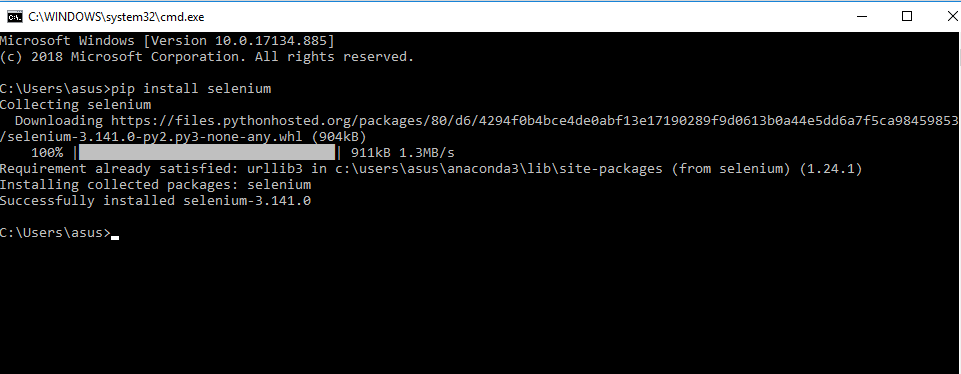
\includegraphics[scale=0.3]{figures/Screenshot_3}
\caption{Installasi Selenium}
\end{figure}
Setelah itu akan muncul tampilan laman Spyder dan langsung isikan code berikut:
\begin{figure}[h]
\centering
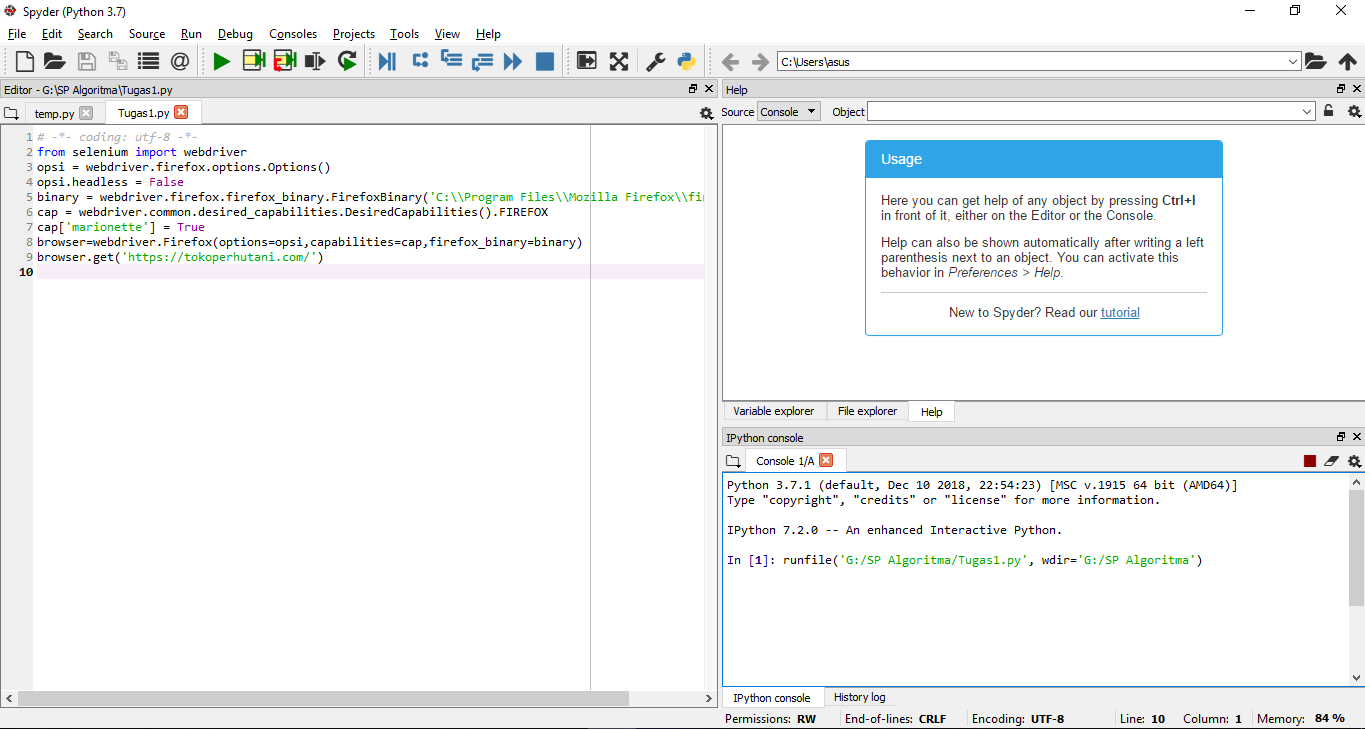
\includegraphics[scale=0.3]{figures/Screenshot_1}
\caption{Code Spyder}
\end{figure}
Jalankan code tersebut hingga muncul seperti ini:
\begin{figure}[h]
\centering
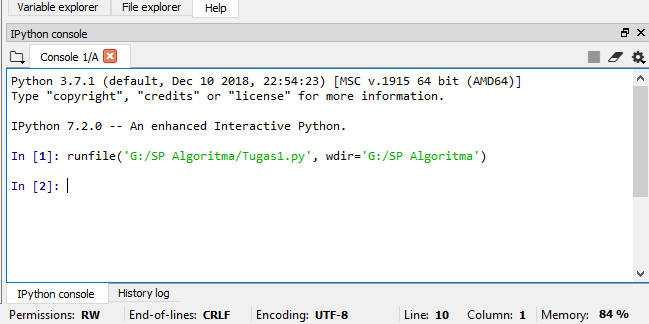
\includegraphics[scale=0.3]{figures/Screenshot_2}
\caption{Running Code di Spyder}
\end{figure}
Selesai! Cek peramban mozilla Anda. Jika muncul web Toko Perhutani, maka installasi berhasil.
\begin{figure}[h]
\centering
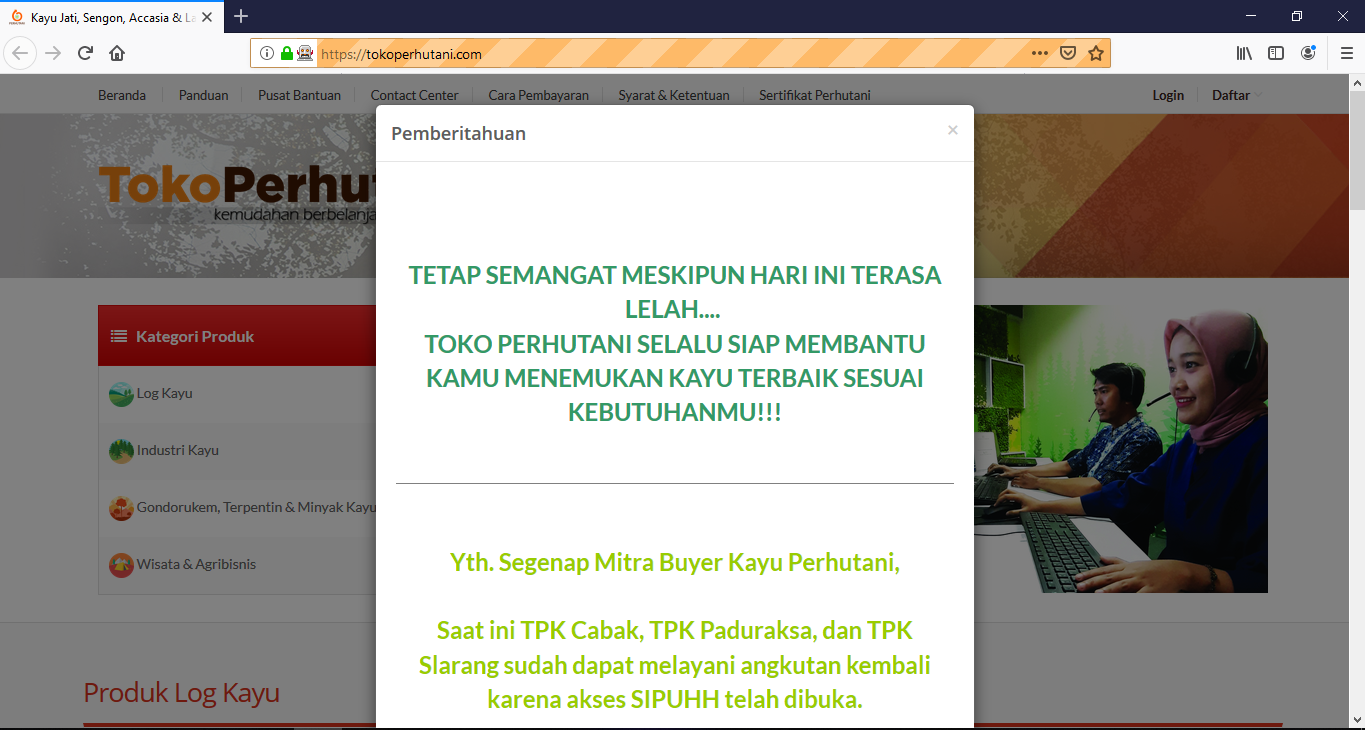
\includegraphics[scale=0.3]{figures/Screenshot_4}
\caption{Laman Web Toko Perhutani}
\end{figure}